\chapter{Infrastruktur}
\label{infrastruktur}
\section{Server in der Cloud mit Amazon EC2}
Die Prämisse war von Anfang an klar: möglichst alle Dienste welche wir für diese Studienarbeit brauchen, sollen aus der \emph{\gls{Cloud}} kommen. Da liegt es natürlich Nahe, dies auch auf die Infrastruktur anzuwenden. Dank dem Amazon Free Usage Tier\footnote{\url{http://aws.amazon.com/free/}} konnten wir kostenlos Server bei Amazon EC2 aufsetzen. Wir haben insgesamt 3 Server aufgesetzt, zwei davon haben wir selbst aufgesetzt und alle Software installiert, bei Redmine konnten wir auf einem bestehenden Image aufsetzen, auf welchem Redmine schon installiert war.

Das Open-Source Projekt BitNami\footnote{\url{http://bitnami.org/}} erstellt für zahlreiche Projekte solche Images. So entfällt ein Grossteil des Installationsaufwand, lediglich zusätzlich gewünschte Plugins müssen noch nachinstalliert werden. Als Benutzer muss ich mich dann nur noch um die Konfiguration kümmern.

\section{Git-Repository bei GitHub}
Wir haben uns für ein Git-Repository entschieden und können somit grundsätzlich unabhängig und offline arbeiten. Als Master für unsere Entwicklung und den Build verwenden wir ein gemeinsames GitHub-Repository\footnote{\url{https://github.com/odi86/GFTPrototype}}.

\begin{figure}[h]
	\centering
	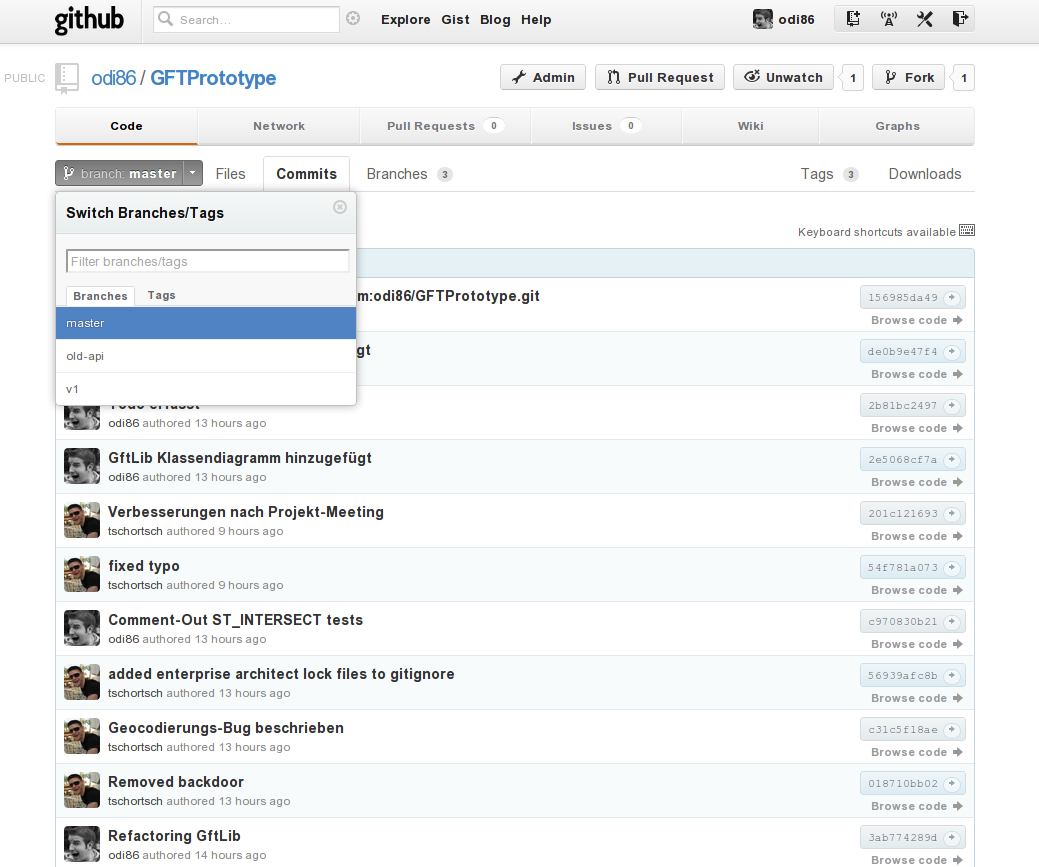
\includegraphics[width=450px]{images/infrastruktur/github-gui}
	\caption{Commit-History in GitHub}
	\label{github-gui}
\end{figure}

Neben dem reinen Repository-Hosting bietet GitHub noch eine Reihe von Zusatzdiensten. Zum Beispiel gibt es einige anschauliche Statistiken über den Code und die Commits. GitHub bietet auch Issues um, mit welchen man Bugs und Feature Requests tracken kann. Daneben bietet die Weboberfläche alles, um das Repository zu durchsuchen, einzelne Files in unterschiedlichen Versionen oder ganze Branches anzuschauen. 

\section{Unit-Testing mit PhantomJS und QUnit}
\todo[inline]{PhantomJS Abschnitt schreiben}

\section{Continuous Integration mit dem Jenkins Build-Server}
Bei Jenkins CI\footnote{\url{http://jenkins-ci.org/}} handelt es sich um ein Open Source Projekt, welches Unterstützung bietet für die Projektautomatisierung. Es unterstützt zahlreiche Repositories und Build-Mechanismen. Wir haben auch einige Plugins aktiviert, u.a. die GitHub- und Redmine-Integration oder der Logfile-Parser.

\subsection{Logfile-Analyse mit dem Log Parser Plugin}
Das Log Parser Plugin\footnote{\url{http://wiki.hudson-ci.org/display/HUDSON/Log+Parser+Plugin}} ermöglicht es auf einfache Art und Weise Probleme mit dem Build festzustellen. Für den Build kann es zum Teil sehr schwierig sein, den Status des Builds zu bestimmen. Der Build kann erkennen ob ein aufgerufener Befehl fehlgeschlagen hat oder ob die ausgeführten Tests erfolgreich durchlaufen. Wenn jedoch ein aufgerufenes Programm eine Warnung oder einen Fehler anzeigt, kann der Build das nicht selbst erkennen. Hier kommt der Logparser ins Spiel. Man kann Muster definieren für Dinge die auf eine Warnung oder einen Fehler hindeuten. Diese Logik erlaubt es dem Build viel detailliertere Aussagen über die laufende Installation zu machen.

\begin{figure}[!h]
	\centering
	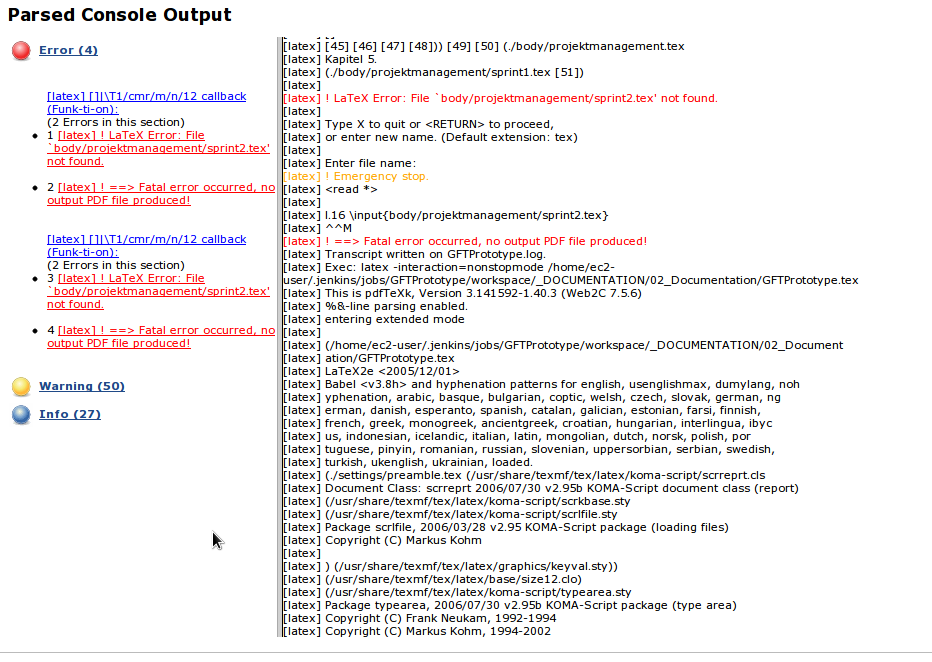
\includegraphics[scale=0.35]{images/infrastruktur/jenkins-parsed-output}
	\caption{Ansicht des Logfiles mit dem Log Parser Plugin}
	\label{jenkins-parsed-output}
\end{figure}

\subsection{Trigger (Auslöser)}
Der Trigger für einen Build ist, wenn eine Änderung auf GitHub gepusht wurde. Dazu haben wir das GitHub Plugin\footnote{\url{https://wiki.jenkins-ci.org/display/JENKINS/Github+Plugin}} auf Jenkins installiert, welches sich einfach im Backend installieren lässt. Im GitHub-Repository mussten wir dann noch sogenannte Web Hooks{\footnote{\url{http://help.github.com/post-receive-hooks/}} einrichten, so dass GitHub jeweils Jenkins benachrichtigt, sobald Änderungen eintreffen.

\subsection{Build Steuerung mit ant}
Zur Build-Steuerung verwenden wir Ant\footnote{\url{http://ant.apache.org/}}. Ant ist vor allem aus der Java-Welt bekannt, lässt sich aber auch gut in andere Umgebungen einbinden. Der Build wir in einer XML-Datei spezifiziert. Einzelne Schritte darin werden \emph{\gls{AntTarget}} genannt und diese sollten grundsätzlich von einander unabhängig sein. Dies ermöglicht es auch nur Teilschritte eines Builds auszuführen. Es lassen sich aber auch Abhängigkeiten zwischen Targets definieren, welche dann der Reihe nach abgearbeitet werden.

Hier zum Beispiel unser \inlinecode{build}-Target, welches alle anderen Targets als Abhängigkeit hat:
\lstset{language=Ant}
\begin{lstlisting}
<target name="build" depends="test,documentation,generate_css,deploy,test-js">
	<echo message="BUILD FINISHED!"/>
</target>
\end{lstlisting}

\subsection{Testausführung}
Zur Darstellung der Testresultate bauen wir auf dem JUnit XML-Interpreter auf, welcher in Jenkins bereits dabei ist. Dazu ist es lediglich notwendig alle Testresultate in das JUnit XML-Format zu bringen, die ganzen Auswertungen, Grafiken etc. bekommt man dann quasi "gratis" dazu.

\begin{figure}[!h]
	\centering
	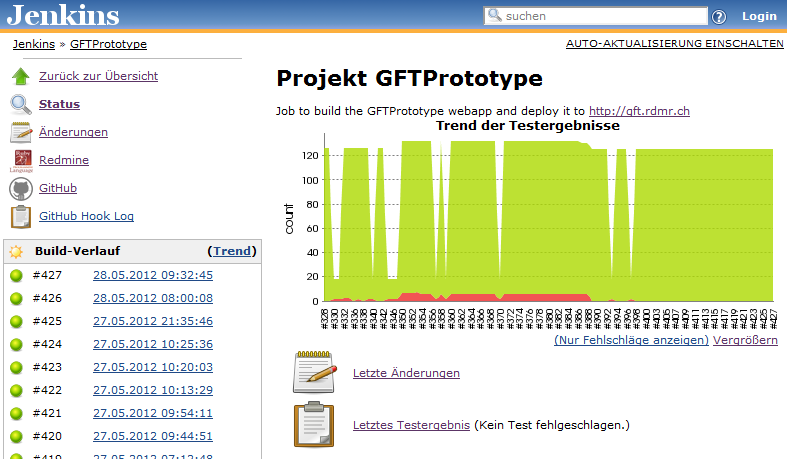
\includegraphics[scale=0.35]{images/infrastruktur/jenkins-test-results}
	\caption{Diagramm der Testresultate im Verlaufe der Zeit}
	\label{jenkins-test-results}
\end{figure}

\section{Projektmanagement mit Redmine}
\todo[inline]{Redmine Abschnitt schreiben}
